 \begin{frame}[fragile]
\frametitle{Data preprocessing: Declarative vs Imperative}

\begin{columns}
\begin{column}{0.5\textwidth}

\large \textbf{Imperative}

\begin{verbatim}
D   vect = CountVectorizer()
A   vect.fit(X)
A   mat = vect.transform(X)
D   rf = RandomForestRegressor()
A   rf.fit(mat, y)
\end{verbatim}

\end{column}
\begin{column}{0.5\textwidth}  %%<--- here

\large \textbf{Declarative}

\begin{verbatim}
D   model = make_pipeline(
D     CountVectorizer(),
D     RandomForestRegressor()
D   )
A   model.fit(X, y)
\end{verbatim}
\end{column}
\end{columns}

\begin{verbatim}
D = declaration, A = action
\end{verbatim}

\end{frame}


\begin{frame}
% When I looked through the kernels during the competition rarely anyone used 
% pipelines to declare models

% for me it is a very important element of building a clean data preprocessing code
% how it works is that first you declare what operations need to happen
% you combine the steps together but in a lazy fashion

% this has its roots in functional programming

\frametitle{"It's pipelines all the way down"}
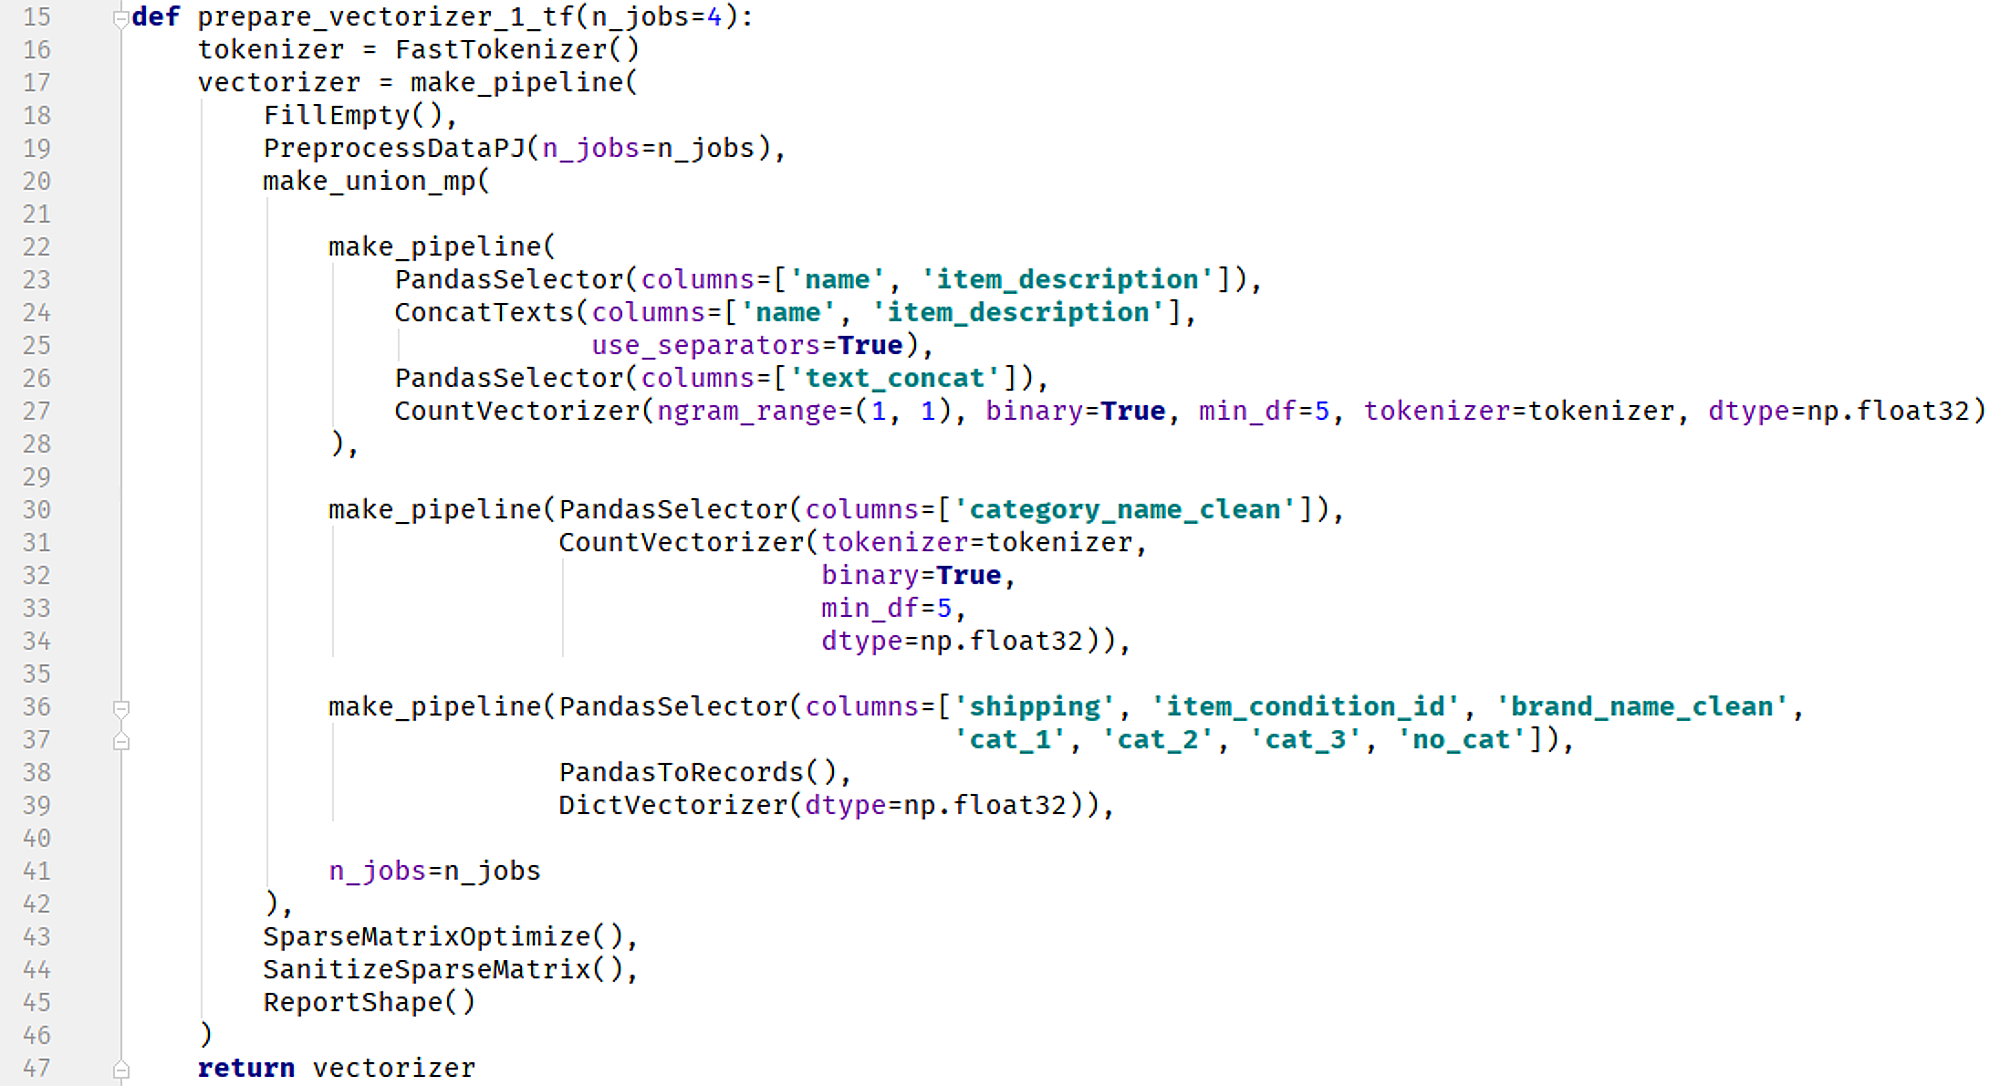
\includegraphics[width=12cm]{img/pipelines-code.png}
\end{frame}


\begin{frame}
\frametitle{Preprocessing}

% we didn't use any magical features
% actually whatever smart features we tried almost none of them worked
% spellchecking, fixing newline bug in the item description
% a proof is in the code golf prepared by Konstantin


\includegraphics[width=1cm]{img/level_expert.png}
\begin{itemize}
\item Text preprocessing - stemming
\item Bag of words - 1,2-grams (with/without Tf-Idf)
\item One hot encoding for categorical columns
\end{itemize}


\includegraphics[width=1cm]{img/level_master.png}
\begin{itemize}
\item Bag of character 3-grams
\end{itemize}


\includegraphics[width=1cm]{img/level_grandmaster.png}
\begin{itemize}
\item Joining name, brand name and description into a single field
\item NumericalVectorizer - vectorizing words using preceding numbers
\end{itemize}

\end{frame}

\begin{frame}
\frametitle{Why ensemble?}

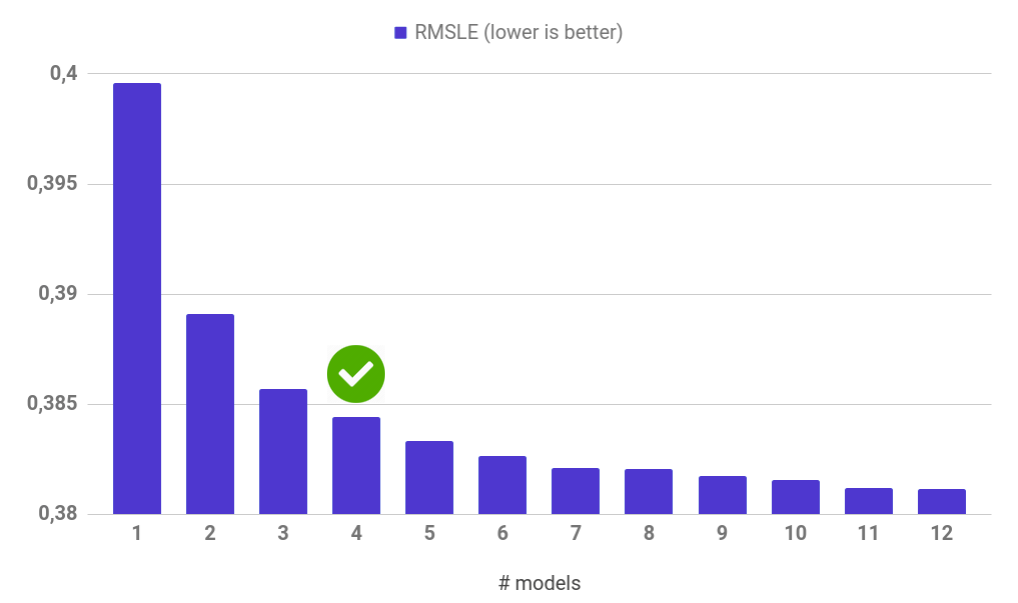
\includegraphics[width=12cm]{img/models_combination.png}

\end{frame}


\begin{frame}
\frametitle{Why 3 datasets?}

% after we merged our solutions it turned out that having 2 datasets
% is much better than 1 dataset
% eventually we used 3 datasets which demanded optimization (overall we spent around 5-minutes of preprocessing per dataset) using ~2 cores on average

% We tried to differentiate the 3 datasets as much as possible
% different stemming (or no stemming)
% unigrams/bigrams

% each new feature was tried in each dataset - some features worked with 1 particular dataset and not in others
% this process was very stochastic

% you can see how the diversity in the datasets improves the result
% the first bar is 4 the same models trained on the 1st dataset.

% you can see how important is to have diverse datasets
% any combination of 2 datasets (8 models) is better than having 12 models

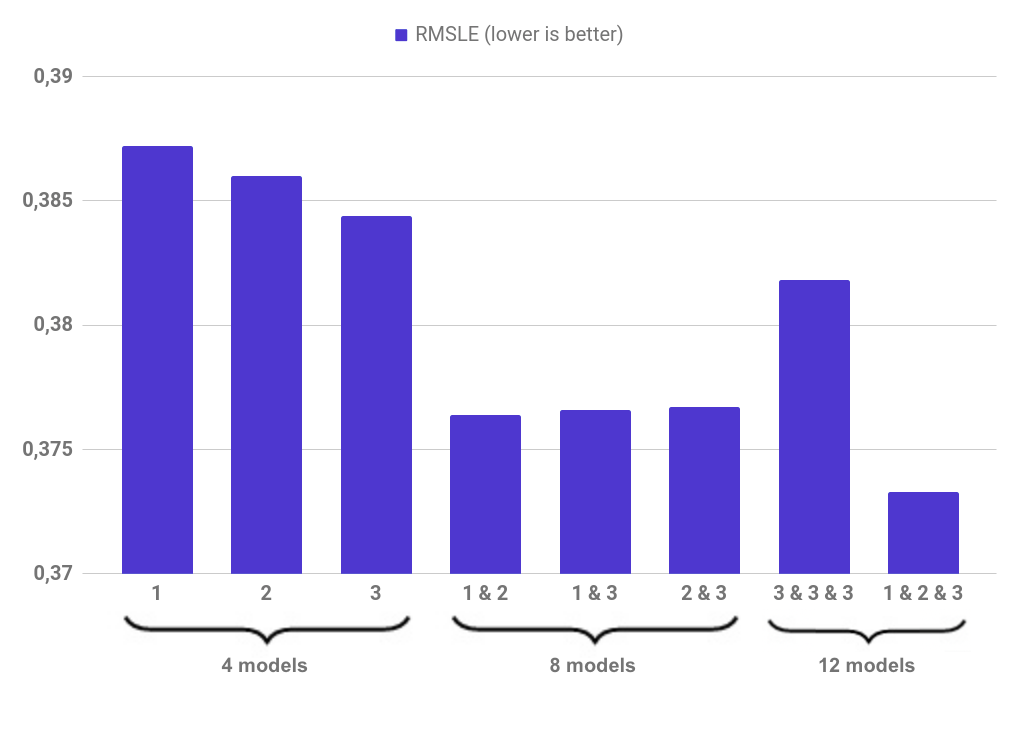
\includegraphics[width=10cm]{img/datasets_combination.png}

\end{frame}